\documentclass{article}


% if you need to pass options to natbib, use, e.g.:
%     \PassOptionsToPackage{numbers, compress}{natbib}
% before loading neurips_2022


% ready for submission
\usepackage{neurips_2022}


% to compile a preprint version, e.g., for submission to arXiv, add add the
% [preprint] option:
%     \usepackage[preprint]{neurips_2022}


% to compile a camera-ready version, add the [final] option, e.g.:
%     \usepackage[final]{neurips_2022}


% to avoid loading the natbib package, add option nonatbib:
%    \usepackage[nonatbib]{neurips_2022}


\usepackage[utf8]{inputenc} % allow utf-8 input
\usepackage[T1]{fontenc}    % use 8-bit T1 fonts
\usepackage{hyperref}
\usepackage{subfigure}
\usepackage{graphicx}    % hyperlinks
\usepackage{url}            % simple URL typesetting
\usepackage{booktabs}       % professional-quality tables
\usepackage{amsfonts}       % blackboard math symbols
\usepackage{nicefrac}       % compact symbols for 1/2, etc.
\usepackage{microtype}      % microtypography
\usepackage{xcolor}         % colors


\title{Self-Supervised Spatial Temporal Feature Learning for Video Correspondence}


% The \author macro works with any number of authors. There are two commands
% used to separate the names and addresses of multiple authors: \And and \AND.
%
% Using \And between authors leaves it to LaTeX to determine where to break the
% lines. Using \AND forces a line break at that point. So, if LaTeX puts 3 of 4
% authors names on the first line, and the last on the second line, try using
% \AND instead of \And before the third author name.


\author{%
  David S.~Hippocampus\thanks{Use footnote for providing further information
    about author (webpage, alternative address)---\emph{not} for acknowledging
    funding agencies.} \\
  Department of Computer Science\\
  Cranberry-Lemon University\\
  Pittsburgh, PA 15213 \\
  \texttt{hippo@cs.cranberry-lemon.edu} \\
  % examples of more authors
  % \And
  % Coauthor \\
  % Affiliation \\
  % Address \\
  % \texttt{email} \\
  % \AND
  % Coauthor \\
  % Affiliation \\
  % Address \\
  % \texttt{email} \\
  % \And
  % Coauthor \\
  % Affiliation \\
  % Address \\
  % \texttt{email} \\
  % \And
  % Coauthor \\
  % Affiliation \\
  % Address \\
  % \texttt{email} \\
}


\begin{document}


\maketitle


\begin{abstract}
  This paper proposes to learn reliable dense correspondence from videos in a self-supervised manner. Our learning process integrates two highly related tasks: tracking large image regions and establishing fine-grained pixel-level associations between consecutive video frames. We exploit the synergy between both tasks through a shared inter-frame affinity matrix, which simultaneously models transitions between video frames at both the region- and pixel-levels. While region-level localization helps reduce ambiguities in fine-grained matching by narrowing down search regions; fine-grained matching provides bottom-up features to facilitate region-level localization. Our method outperforms the state-of-the-art self-supervised methods on a variety of visual correspondence tasks, including video-object and part-segmentation propagation, keypoint tracking, and object tracking. Our self-supervised method even surpasses the fully-supervised affinity feature representation obtained from a ResNet-18 pre-trained on the ImageNet.
\end{abstract}


\section{Introduction}
Learning representations for video correspondence is a fundamental problem in computer vision, which is closely related to different video applications including optical flow estimation, video object segmentation, and keypoint tracking, etc. However, supervising such a representation requires a big amount of dense annotations which is unaffordable. Thus most approaches acquire supervision from simulations or limited annotations, which result in poor generalization in different downstream tasks. Recently, self-supervised feature learning is gaining significant momentum, and a number of pretext tasks are designed for space-time visual correspondence using abundant unlabeled videos. \\
\\
The key to this task lies in two different perspectives. The first one is \textbf{temporal feature learning}, which aims to learn the displacement of pixel/object between frames. With the the nature of temporal coherence in video, the temporal feature learning can be formed as a reconstruction task, where the query pixel in target frame can be reconstructed by leavraging the information of adjacent reference frames within a local region. Then a reconstruction loss is applied for minimizing the photometric error between the raw frame and its reconstruction [1][2]. However, in real videos, the temporal discontinuity occurs frequently due to the occlusions, illumination changes, and deformations especially for pixels in each frame with severe down-sampling. In such scenarios, the frame reconstruction loss apparently becomes invalid. To alleviate the problem, MAST[1] propose to apply frame reconstruction with a higher feature resolution by decrease the stride of backbone, which requires a larger memory and computation cost. Another way to exploit the free temporal supervision is applying object-level reconstruction. [3] track object forward and backward with the objective of maximizing the temporal cycle correspondence consistency with reconstruction loss. However, compared to object-level reconstruction which need a extra localization module, the frame reconstruction is conducted on raw image space, which provide more accurate supervision for learning fine-grained correspondence.\\
\\
The second one is \textbf{spatial feature learning}, which pays more attention to learning the object appearance that is invariant to viewpoint and deformation changes.  [4] adopt a novel intra-inter consistency loss to learn inter-video discriminative feature. [5] learn the space-time correspondence through a frame-wise contrastive loss. However, both methods are trained on video dataset and try to realize the spatial and temporal feature learning in a unified framework, which is sub-optimal for each of them. Recently, the contrastive model  pre-trained on image data show impressive performance for dense representation. This motivates us to design a framework that learn the spatial and temporal feature independently with image and video data.  \\
\\
In this paper, we decouple video correspondence learning into two separate process including spatial and temporal feature learning. To achieve this, we first train the model in a contrastive learning paradigm on ImageNet, which gives the model the ability of capturing object appearance. Then, instead of training with a large video dataset, i.e., Kinetics[4] with 300k videos, we perform the temporal feature learning on YouTube-VOS which consists of 3.5k videos. However, apart from the severe temporal discontinuity due to large spatial down-sampling on frames, directly fine-tuning the old model with only new data will lead to a well-known phenomenon of catastrophic forgetting, which degrades the performance. To address both problems, we propose a novel pyramid learning framework. We first apply the frame reconstruction at different layers of pyramid network to better exploit the free temporal supervision. The pixels of target and reference frame with  higher resolution have lower chance of occurring temporal discontinuity, which may result in more accurate local correlation map. Thus we design a new loss named local correlation distillation loss that supports explicitly learning of the network output by taking the finest local correlation map as pseudo labels. On the other hand, since the model pre-trained on ImageNet.


% \begin{figure}[!tb]
%   \centering
%   \subfigure[\scriptsize Temporal Feature Learning]{
%     \label{fig:motion_map:a}
%     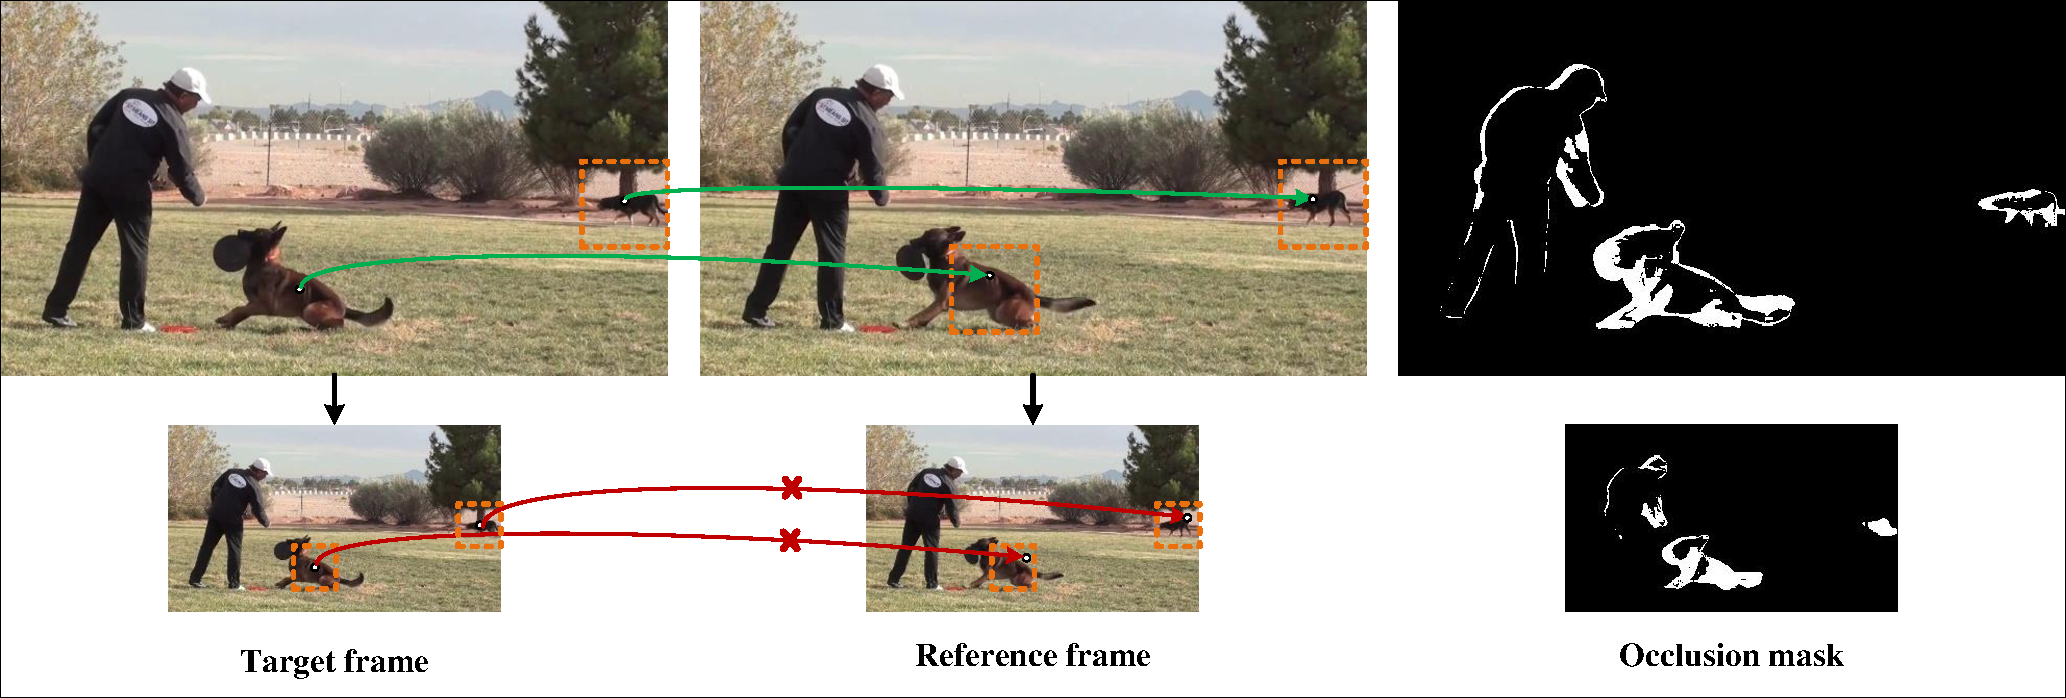
\includegraphics[width=1.0\textwidth]{figure/tissor/tissor.pdf}}
%   % \hspace{0.1in}
%   \subfigure[\scriptsize Spatial Feature Learning]{
%     \label{fig:motion_map:b}
%     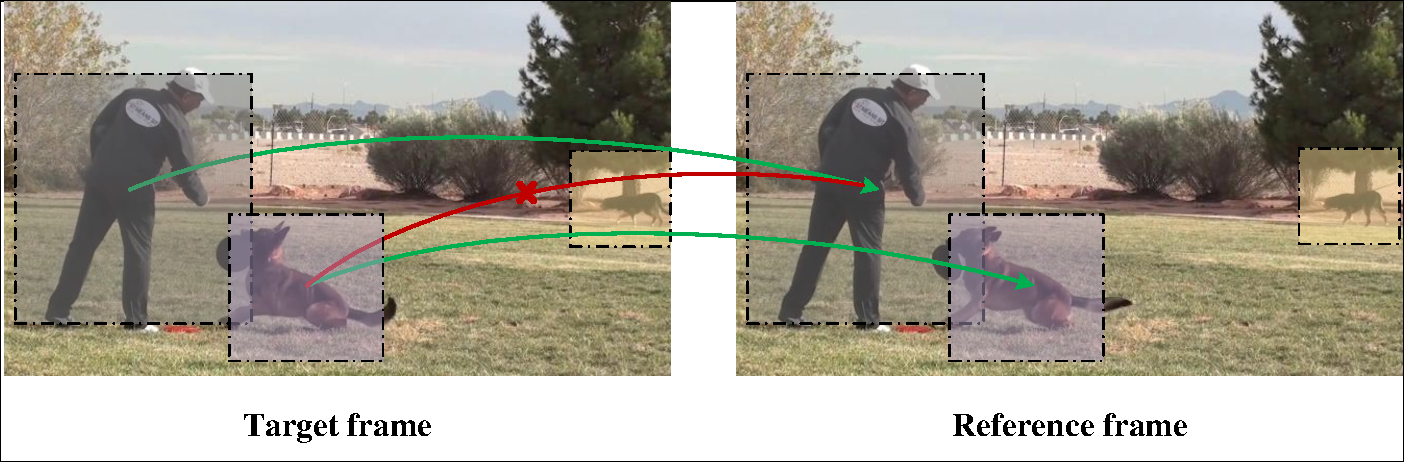
\includegraphics[width=1.0\textwidth]{figure/tissor/tissor2.pdf}}
%   \caption{\small The example of (a) input video sequence, (b) optical flow, (c) motion boundary, (d) motion map, (e) valuable mutual information in the region with large movement and (f) nuisance mutual information in the relatively static region. The red box and green box represent two views generated from the identical instance for contrastive learning.}
%   \label{fig:motion_map}
% \end{figure}
\begin{figure}[!tb]
  \centering
  {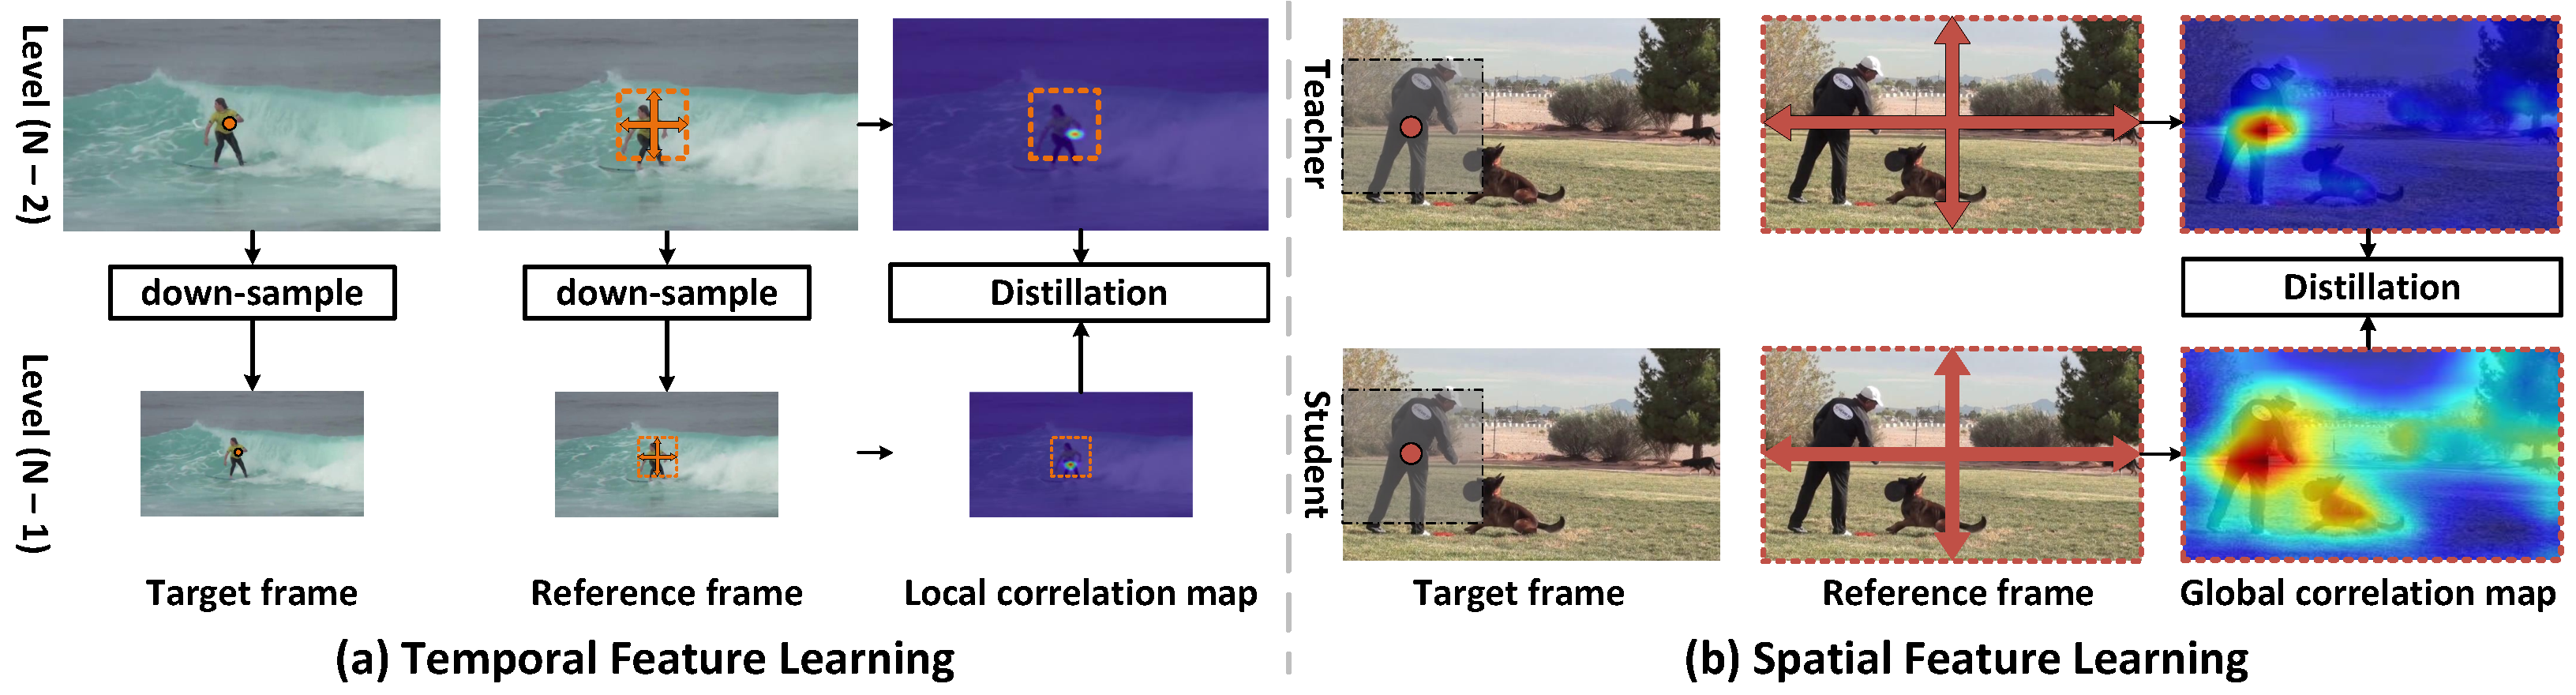
\includegraphics[width=1.0\textwidth]{figure/tissor/tissor6.pdf}}
  \caption{\small The example of (a) input video sequence, (b) optical flow, (c) motion boundary, (d) motion map, (e) valuable mutual information in the region with large movement and (f) nuisance mutual information in the relatively static region.}
  \label{fig:tissor}
\end{figure}

\section{Related Work}
\textbf{Object-level correspondence.} The goal of visual tracking is to determine a bounding box in each frame based on an annotated box in the reference image. Most methods belong to one of the two categories that use: (a) the tracking-by-detection framework [1, 20, 46, 25], which models tracking as detection applied independently to individual frames; or (b) the tracking-by-matching framework that models cross-frame relations and includes several early attempts, e.g., mean-shift trackers [8, 54], kernelized correlation filters (KCF) [14, 27], and several works that model correlation filters as differentiable blocks [32, 33, 7, 47]. Most of these methods use annotated bounding boxes [52] in every frame of the videos to learn feature representations for tracking. Our work can be viewed as exploiting the tracking-by-matching framework in a self-supervised manner. \\
\\
\textbf{Fine-grained correspondence.} Dense correspondence between video frames has been widely applied for optical flow and motion estimation [31, 40, 29, 16], where the goal is to track individual pixels. Most deep neural networks [16, 40] are trained with the objective of regressing the groundtruth optical flow produced by synthetic datasets [4, 10]. In contrast to many classic methods [31, 29] that model dense correspondence as a matching problem, direct regression of pixel offsets has limited capability for frames containing dramatic appearance changes [3, 39], and suffers from problems related to domain shift when applied to real-world scenarios.

\textbf{Self-supervised learning.} Recently, numerous approaches have been developed for correspondence learning via various self-supervised signals, including image [17] or color transformation [44] and cycle-consistency [51, 45]. Self-supervised learning of correspondence in videos has been explored along the two different directions – for region-level localization [51, 45] and for fine-grained pixel level matching [44, 23]. In [45], a correlation filter is learned to track regions via a cycle-consistency constraint, and no pixel-level correspondence is determined. [51] develops patch-level tracking by modeling the similarity transformation of pixels within a fixed rectangular region. Conversely, several methods learn a matching network by transforming color/RGB information between adjacent frames [44, 24, 23]. As no region-level regularization is exploited, these approaches are less effective when color features are less distinctive (see Figure 1(b)). In contrast, our method learns object-level and pixel-level correspondence jointly across video frames in a self-supervised manner.


\section{Approach}



\section{Experiments}



\section{Conclusions}



\section*{References}
\medskip


{
\small


[1] Alexander, J.A.\ \& Mozer, M.C.\ (1995) Template-based algorithms for
connectionist rule extraction. In G.\ Tesauro, D.S.\ Touretzky and T.K.\ Leen
(eds.), {\it Advances in Neural Information Processing Systems 7},
pp.\ 609--616. Cambridge, MA: MIT Press.


[2] Bower, J.M.\ \& Beeman, D.\ (1995) {\it The Book of GENESIS: Exploring
  Realistic Neural Models with the GEneral NEural SImulation System.}  New York:
TELOS/Springer--Verlag.


[3] Hasselmo, M.E., Schnell, E.\ \& Barkai, E.\ (1995) Dynamics of learning and
recall at excitatory recurrent synapses and cholinergic modulation in rat
hippocampal region CA3. {\it Journal of Neuroscience} {\bf 15}(7):5249-5262.
}


%%%%%%%%%%%%%%%%%%%%%%%%%%%%%%%%%%%%%%%%%%%%%%%%%%%%%%%%%%%%
\section*{Checklist}


%%% BEGIN INSTRUCTIONS %%%
The checklist follows the references.  Please
read the checklist guidelines carefully for information on how to answer these
questions.  For each question, change the default \answerTODO{} to \answerYes{},
\answerNo{}, or \answerNA{}.  You are strongly encouraged to include a {\bf
justification to your answer}, either by referencing the appropriate section of
your paper or providing a brief inline description.  For example:
\begin{itemize}
  \item Did you include the license to the code and datasets? \answerYes
  \item Did you include the license to the code and datasets? \answerNo{The code and the data are proprietary.}
  \item Did you include the license to the code and datasets? \answerNA{}
\end{itemize}
Please do not modify the questions and only use the provided macros for your
answers.  Note that the Checklist section does not count towards the page
limit.  In your paper, please delete this instructions block and only keep the
Checklist section heading above along with the questions/answers below.
%%% END INSTRUCTIONS %%%


\begin{enumerate}


\item For all authors...
\begin{enumerate}
  \item Do the main claims made in the abstract and introduction accurately reflect the paper's contributions and scope?
    \answerTODO{}
  \item Did you describe the limitations of your work?
    \answerTODO{}
  \item Did you discuss any potential negative societal impacts of your work?
    \answerTODO{}
  \item Have you read the ethics review guidelines and ensured that your paper conforms to them?
    \answerTODO{}
\end{enumerate}


\item If you are including theoretical results...
\begin{enumerate}
  \item Did you state the full set of assumptions of all theoretical results?
    \answerTODO{}
        \item Did you include complete proofs of all theoretical results?
    \answerTODO{}
\end{enumerate}


\item If you ran experiments...
\begin{enumerate}
  \item Did you include the code, data, and instructions needed to reproduce the main experimental results (either in the supplemental material or as a URL)?
    \answerTODO{}
  \item Did you specify all the training details (e.g., data splits, hyperparameters, how they were chosen)?
    \answerTODO{}
        \item Did you report error bars (e.g., with respect to the random seed after running experiments multiple times)?
    \answerTODO{}
        \item Did you include the total amount of compute and the type of resources used (e.g., type of GPUs, internal cluster, or cloud provider)?
    \answerTODO{}
\end{enumerate}


\item If you are using existing assets (e.g., code, data, models) or curating/releasing new assets...
\begin{enumerate}
  \item If your work uses existing assets, did you cite the creators?
    \answerTODO{}
  \item Did you mention the license of the assets?
    \answerTODO{}
  \item Did you include any new assets either in the supplemental material or as a URL?
    \answerTODO{}
  \item Did you discuss whether and how consent was obtained from people whose data you're using/curating?
    \answerTODO{}
  \item Did you discuss whether the data you are using/curating contains personally identifiable information or offensive content?
    \answerTODO{}
\end{enumerate}


\item If you used crowdsourcing or conducted research with human subjects...
\begin{enumerate}
  \item Did you include the full text of instructions given to participants and screenshots, if applicable?
    \answerTODO{}
  \item Did you describe any potential participant risks, with links to Institutional Review Board (IRB) approvals, if applicable?
    \answerTODO{}
  \item Did you include the estimated hourly wage paid to participants and the total amount spent on participant compensation?
    \answerTODO{}
\end{enumerate}


\end{enumerate}


%%%%%%%%%%%%%%%%%%%%%%%%%%%%%%%%%%%%%%%%%%%%%%%%%%%%%%%%%%%%


\appendix


\section{Appendix}


Optionally include extra information (complete proofs, additional experiments and plots) in the appendix.
This section will often be part of the supplemental material.


\end{document}